\section{Methodology}
In this section we highlight the underlying methodology and steps involved in this paper. The entire methodology can be broadly classified into three phases as shown in the figure \ref{fig:flow-diagram}, namely: i) Data collection, ii) Training and iii) Testing/ evaluation.

\subsection{Data Collection}
As defined in the section \ref{sec:PDMORL}, a data sample for any RL method consists of state, action, next state and reward. The state is a representative of the environment and the agents action on it. The RL agent constantly observe this state and take action a(t) based on the observation that results in the environment transition from state s(t) to the state s(t+1) while returning the reward r(t). The HPC node environment is defined by the hardware and the application that runs on it. Therefore we use the features engineered using the measurements from hardware performance counters along with progress and measured power as the representative of the state. Apart from these we also give the user defined decay in performance as one of the feature of the state. Therefore $s(t) = [progress(t), power(t), IPC(t), STL(t), CMR(t), d(t)] \in \mathbb{R}^{6}$. The action $a(t)$ in case of the HPC node is the node power cap represented as $PCAP(t) \in \mathbb{R}$. Reward in case of a multiobjective reinforcement learning is not any more scalar. Rather it is a vector whose dimension equals the number of objectives. In our case, energy and execution time being two objectives deciding the pareto front our reward vector $\mathbf{r}(t) = [progress, power]$ as defined in the equation \ref{eq:reward_vector}. As the underlying learning is going to be offline it is important to include optimal policies in the dataset. As all actions are optimal corresponding to some decay factor $d(t_i)$ we calculate the delta from the collected data set. We calculate the delta using the equation \ref{eq:decay} and append it to the state of the dataset. Followingly, the state $s(t)$ and the next state $s(t+1)$ are both appended with the calculated decay to ensure a sequential state transition.  

\subsection{Offline Training}
We use offline reinforcement learning to avoid the training model and run time application compete for the same node resources \ref{sec:Introduction}. The dataset collected is now used to train an RL agent defined using a Q network. The state observation consisting of the $s(t) = [progress(t), power(t), IPC(t), STL(t), CMR(t), d(t)]$ goes into a finite action spaced Q network and return the Q vector corresponding to each of the actions defined in the action space. This Q vector is compared against a weight vector calculated using the data points connecting the PCAP and progress for alignment and also evaluated for maximum performance per watt.  

\begin{algorithm}[t]
\caption{Offline Preference-Aligned Q-Learning}
\label{alg:offline_pref_qlearning}
\begin{algorithmic}[1]
\Require Offline dataset $\mathcal{D}=\{(s_t,a_t,r_t,s_{t+1})\}$
\Require Progress--PCAP model $\mathcal{G}_{app}$
\Require Learning rate $\eta$, discount $\gamma$, batch size $B$, soft update rate $\tau$
\Ensure Trained network parameters $\theta$

\State Initialize online network $Q_\theta$ and target network $Q_{\bar{\theta}} \leftarrow Q_\theta$

\For{each iteration}
    \State Sample minibatch $\{(s_i,a_i,r_i,s'_i)\}_{i=1}^B \sim \mathcal{D}$
    
    \State Construct state $s_i = [progress, power, IPC, STL, CMR, d]$
    
    \State Compute decay-aligned target progress:
    \[
    g_i^* = (1-\delta_i)\, g_{\max}
    \]
    
    \State Map to desired PCAP:
    \[
    \text{PCAP}_{\text{des},i} = \mathcal{G}_{app}(g_i^*)
    \]
    
    \State Construct aligned preference vector $\boldsymbol{\omega}_i$
    
    \State Compute target using preference-aware Bellman operator:
    \begin{equation*}
    (\mathcal{T}\mathbf{Q})(s,a,\boldsymbol{\omega})
    = \mathbf{r}(s,a)
    + \gamma \mathbb{E}_{s' \sim P(\cdot \mid s,a)} \Big[
    \mathbf{Q}\Big(
    s',
    \arg\max_{a' \in \mathcal{A}}
    \big(
    S_c(\boldsymbol{\omega}, \mathbf{Q}(s',a',\boldsymbol{\omega}))
    \cdot
    \boldsymbol{\omega}^{\top} \mathbf{Q}(s',a',\boldsymbol{\omega})
    \big),
    \boldsymbol{\omega}
    \Big)
    \Big]
    \end{equation*}
    
    \State Approximate expectation using sampled $s'_i$ and target network $Q_{\bar{\theta}}$
    
    \State Form Bellman target:
    \[
    y_i = (\mathcal{T}\mathbf{Q})(s_i,a_i,\boldsymbol{\omega}_i)
    \]
    
    \State Update network parameters:
    \[
    \theta \leftarrow \theta - \eta \nabla_\theta
    \frac{1}{B}\sum_{i=1}^B \left\|Q_\theta(s_i,a_i)-y_i\right\|^2
    \]
    
    \State Soft update target network:
    \[
    \bar{\theta} \leftarrow \tau \theta + (1-\tau)\bar{\theta}
    \]
    
\EndFor

\State \Return $Q_\theta$
\end{algorithmic}
\end{algorithm}

\subsection{Evaluation}

For the evaluation phase we use the trained model and deploy it alongside the runtime applications on the hardware having similar actuator configuration.  We perform the evaluation using different applications as given in the table \ref{tab:performance_metrics} that differentiates training and testing applications. During the evaluation the controller receives information from the hardware performance counters that are instantaneously converted to the useful features along with progress and average power consumed. Followingly we append the user defined preference to this feature vector and let the controller implement the action. The action is enforced using the PCAP control knob through the intel RAPL actuators. We repeat the process multiple times and record the average of energy and execution time to get a good repeatability statistics. We evaluate the results by plotting the pareto front of the application on a given hardware alongside the proposed controller. We plot the weigtage or the preferences on each of the objectives for the points obtained as well as the percentage decay each of these points corresponds to.

\begin{figure}[tbp]
    \centering
    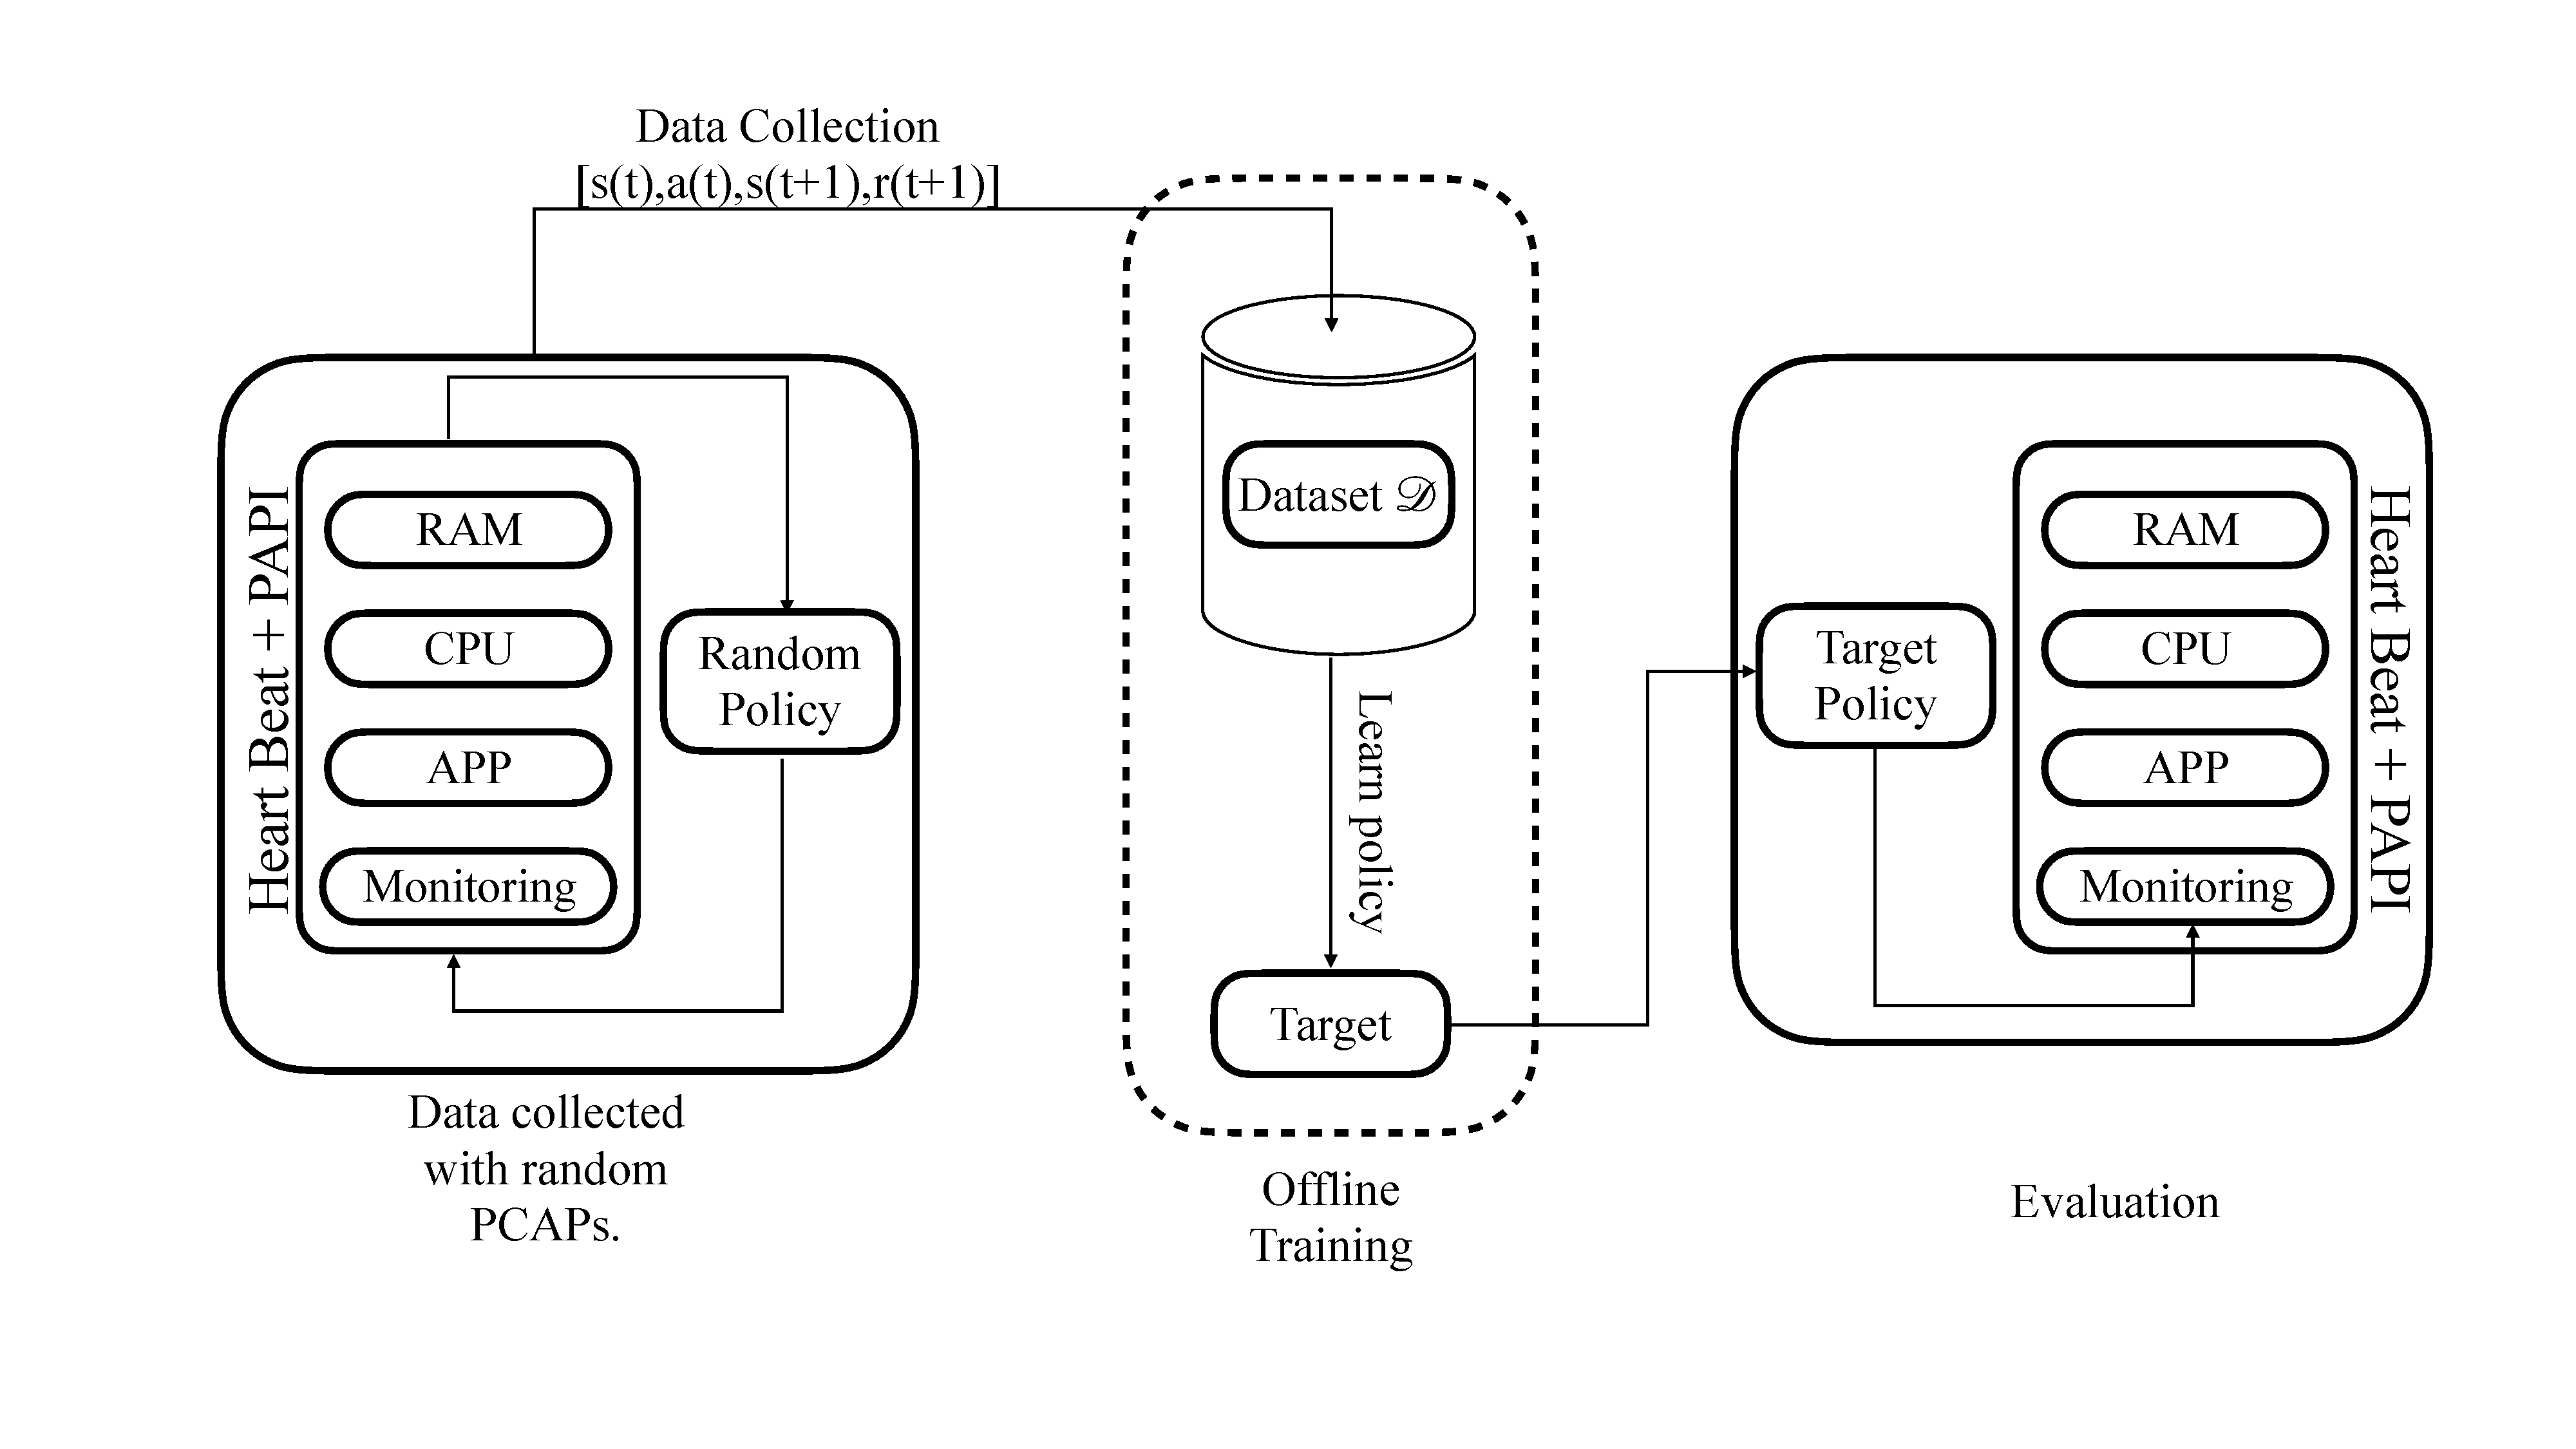
\includegraphics[width=\linewidth,trim=5.5cm 6cm 3cm 1cm]{Figure/block_diagram.pdf}
    \caption{{Flow diagram for offline reinforcement learning: data is collected using an arbitrary policy to train the agent without system access, and the trained agent is later deployed for evaluation. Note that the lines in the diagram are not closed to form a loop, indicating offline training and online testing.}}
    \label{fig:flow-diagram}
%    \Description{Flow diagram of methodology}
\end{figure}

